% Hlavicka pro protokoly z fyzikalniho praktika.
% Verze pro: LaTeX
% Verze hlavicky: 22. 2. 2007
% Autor: Ustav fyziky kondenzovanych latek
% Ke stazeni: www.physics.muni.cz/ufkl/Vyuka/
% Licence: volne k pouziti, nejlepe k vcasnemu odevzdani protokolu z Vaseho mereni.


\documentclass[czech,11pt,a4paper]{article}
\usepackage[T1]{fontenc}
\usepackage{graphicx, animate}
\usepackage{mathtools}
\usepackage{amssymb}
\usepackage{amsthm}
\usepackage{thmtools}
\usepackage{xcolor}
\usepackage{nameref}
\usepackage{babel}
\usepackage{hyperref}
\usepackage{multicol}
\usepackage[export]{adjustbox}
\usepackage{subcaption}
\usepackage{caption}
\usepackage{multirow}
\usepackage{float}
\usepackage{placeins}
\usepackage{biblatex}
\graphicspath{ {./images/} }




%%% Nemente:
\usepackage[margin=2cm]{geometry}
\newtoks\jmenopraktika \newtoks\jmeno \newtoks\datum
\newtoks\obor \newtoks\skupina \newtoks\rocnik \newtoks\semestr
\newtoks\cisloulohy \newtoks\jmenoulohy
\newtoks\tlak \newtoks\teplota \newtoks\vlhkost
%%% Nemente - konec.


%%%%%%%%%%% Doplnte pozadovane polozky:

\jmenopraktika={Fyzikální praktikum 2}  % nahradte jmenem vaseho predmetu
\jmeno={Teodor Duraković}            % nahradte jmenem mericiho
\datum={11.~listopadu 2024}        % nahradte datem mereni ulohy
\obor={F}                     % nahradte zkratkou vami studovaneho oboru
\skupina={Po 14:00}            % nahradte dobou vyuky vasi seminarni skupiny
\rocnik={II}                  % nahradte rocnikem, ve kterem studujete
\semestr={III}                 % nahradte semestrem, ve kterem studujete

\cisloulohy={6}               % nahradte cislem merene ulohy
\jmenoulohy={Elektromagnetické kmity v RLC obvodu} % nahradte jmenem merene ulohy

\tlak={1002}                   % nahradte tlakem pri mereni (v hPa)
\teplota={21.9}               % nahradte teplotou pri mereni (ve stupnich Celsia)
\vlhkost={45}               % nahradte vlhkosti vzduchu pri mereni (v %)

%%%%%%%%%%% Konec pozadovanych polozek.


%%%%%%%%%%% Uzitecne balicky:

%%%%%% Zamezeni parchantu:
\widowpenalty 10000 \clubpenalty 10000 \displaywidowpenalty 10000
%%%%%% Parametry pro moznost vsazeni vetsiho poctu obrazku na stranku
\setcounter{topnumber}{3}	  % max. pocet floatu nahore (specifikace t)
\setcounter{bottomnumber}{3}	  % max. pocet floatu dole (specifikace b)
\setcounter{totalnumber}{6}	  % max. pocet floatu na strance celkem
\renewcommand\topfraction{0.9}	  % max podil stranky pro floaty nahore
\renewcommand\bottomfraction{0.9} % max podil stranky pro floaty dole
\renewcommand\textfraction{0.1}	  % min podil stranky, ktery musi obsahovat text
\intextsep=8mm \textfloatsep=8mm  %\intextsep pro ulozeni [h] floatu a \textfloatsep pro [b] or [t]

% Tecky za cisly sekci:
\renewcommand{\thesection}{\arabic{section}.}
\renewcommand{\thesubsection}{\thesection\arabic{subsection}.}
\renewcommand{\thesubsubsection}{\thesubsection\arabic{subsubsection}.}
% Jednopismenna mezera mezi cislem a nazvem kapitoly:
\makeatletter \def\@seccntformat#1{\csname the#1\endcsname\hspace{1ex}} \makeatother


%%%%%%%%%%%%%%%%%%%%%%%%%%%%%%%%%%%%%%%%%%%%%%%%%%%%%%%%%%%%%%%%%%%%%%%%%%%%%%%
%%%%%%%%%%%%%%%%%%%%%%%%%%%%%%%%%%%%%%%%%%%%%%%%%%%%%%%%%%%%%%%%%%%%%%%%%%%%%%%
% Zacatek dokumentu
%%%%%%%%%%%%%%%%%%%%%%%%%%%%%%%%%%%%%%%%%%%%%%%%%%%%%%%%%%%%%%%%%%%%%%%%%%%%%%%
%%%%%%%%%%%%%%%%%%%%%%%%%%%%%%%%%%%%%%%%%%%%%%%%%%%%%%%%%%%%%%%%%%%%%%%%%%%%%%%

\begin{document}
	
	%%%%%%%%%%%%%%%%%%%%%%%%%%%%%%%%%%%%%%%%%%%%%%%%%%%%%%%%%%%%%%%%%%%%%%%%%%%%%%%
	% Nemente:
	%%%%%%%%%%%%%%%%%%%%%%%%%%%%%%%%%%%%%%%%%%%%%%%%%%%%%%%%%%%%%%%%%%%%%%%%%%%%%%%
	\thispagestyle{empty}
	
	{
		\begin{center}
			\sf 
			{\Large Ústav fyzikální elektroniky Přírodovědecké fakulty Masarykovy univerzity} \\
			\bigskip
			{\huge \bfseries FYZIKÁLNÍ PRAKTIKUM} \\
			\bigskip
			{\Large \the\jmenopraktika}
		\end{center}
		
		\bigskip
		
		\sf
		\noindent
		\setlength{\arrayrulewidth}{1pt}
		\begin{tabular*}{\textwidth}{@{\extracolsep{\fill}} l l}
			\large {\bfseries Zpracoval:}  \the\jmeno & \large  {\bfseries Naměřeno:} \the\datum\\[2mm]
			\large  {\bfseries Obor:} \the\obor  \hspace{40mm}  {\bfseries Skupina:} \the\skupina %
			%{\bfseries Ročník:} \the\rocnik \hspace{5mm} {\bfseries Semestr:} \the\semestr  
			&\large {\bfseries Testováno:}\\
			\\
			\hline
		\end{tabular*}
	}
	
	\bigskip
	
	{
		\sf
		\noindent \begin{tabular}{p{3cm} p{0.6\textwidth}}
			\Large  Úloha č. {\bfseries \the\cisloulohy:} \par
			\smallskip
			$T=\the\teplota$~$^\circ$C \par
			$p=\the\tlak$~hPa \par
			$\varphi=\the\vlhkost$~\%
			&\Large \bfseries \the\jmenoulohy  \\[2mm]
		\end{tabular}
	}
	
	\vskip1cm
	
	%%%%%%%%%%%%%%%%%%%%%%%%%%%%%%%%%%%%%%%%%%%%%%%%%%%%%%%%%%%%%%%%%%%%%%%%%%%%%%%
	% konec Nemente.
	%%%%%%%%%%%%%%%%%%%%%%%%%%%%%%%%%%%%%%%%%%%%%%%%%%%%%%%%%%%%%%%%%%%%%%%%%%%%%%%
	
	%%%%%%%%%%%%%%%%%%%%%%%%%%%%%%%%%%%%%%%%%%%%%%%%%%%%%%%%%%%%%%%%%%%%%%%%%%%%%%%
	%%%%%%%%%%%%%%%%%%%%%%%%%%%%%%%%%%%%%%%%%%%%%%%%%%%%%%%%%%%%%%%%%%%%%%%%%%%%%%%
	% Zacatek textu vlastniho protokolu
	%%%%%%%%%%%%%%%%%%%%%%%%%%%%%%%%%%%%%%%%%%%%%%%%%%%%%%%%%%%%%%%%%%%%%%%%%%%%%%%
	%%%%%%%%%%%%%%%%%%%%%%%%%%%%%%%%%%%%%%%%%%%%%%%%%%%%%%%%%%%%%%%%%%%%%%%%%%%%%%%
	
	\begin{multicols}{2}
		\section{Zadání}
		1. Určit impedanci resistoru, kondenzátoru a cívky.\\
		2. Změřit frekvenční charakteristiku buzeného RLC obvodu a určit z nich odpor, indukci a kapacitu RLC obvodu.
		\\
		3. Změřit přechodový jev (vlastní kmity) RLC obvodu s podkritickým, kritickým a nadkritickým tlumením, a určit vlastní frekvenci obvodu a koeficient útlumu.
		
		\section{Úvod}
		Uvažujme obvod, kde jsou prvky R, L a C řazené v sérii, viz obr. 1, a jsou buzeny napětím z funkčního generátoru $U(t)$. Druhý Kirchhoffův zákon říká, že součet úbytků napětí na spotřebičích se v uzavřeném obvodě rovná součtu napětí na zdrojích. V případě tohoto obvodu tedy nabývá tvar
		\begin{equation}
			U_{R}(t)+U_{L}(t)+U_{C}(t)=U(t)
		\end{equation}
		
		\begin{figure}[H]
			\begin{center}
				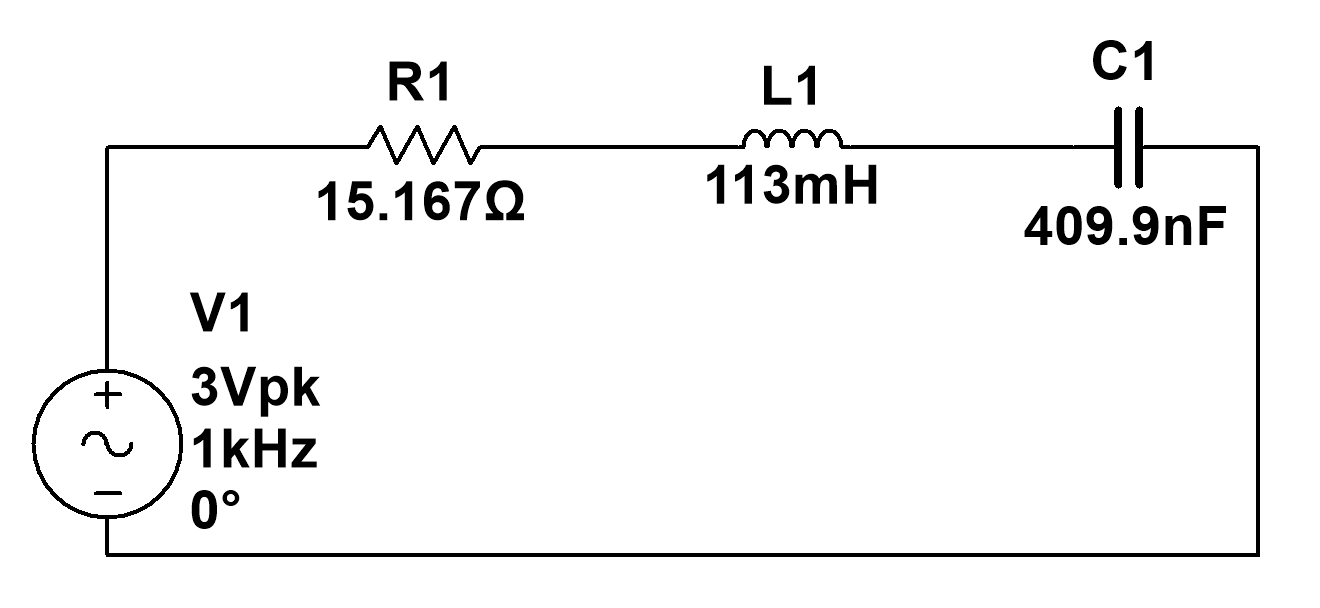
\includegraphics[max width=0.9\linewidth, center]{obvod1}
				\caption{Schéma RLC obvodu s prvky zapojenými v sérii}
				
			\end{center}
		\end{figure}
		formuli (1) lze podle Ohmova, Faradayova a Coulombova zákona upravit na
		\begin{equation}
			L \frac{\mathrm{~d}^{2} I(t)}{\mathrm{d} t^{2}}+R \frac{\mathrm{~d} I(t)}{\mathrm{d} t}+\frac{1}{C} I(t)=\frac{\mathrm{d} U(t)}{\mathrm{d} t}.
		\end{equation}
		Stacionární řešení, platí-li pro proud a napětí na zdroji
		\begin{equation}
			\hat{U}(t)=\hat{U}_{0}(\omega) \mathrm{e}^{\mathrm{i} \omega t}, \quad \hat{I}(t)=\hat{I}_{0}(\omega) \mathrm{e}^{\mathrm{i} \omega t},
		\end{equation}
		při zapojení pouze odporu, cívky nebo kapacity, budou vypadat následovně:
		\subsection{Obvod s odporem}
		Rovnice (1) se nám redukuje na
		\begin{equation}
			R I =U
		\end{equation}
		a po dosazení formule (3) získáváme
		\begin{equation}
			R \hat{I}_{0}(\omega)=\hat{U}_{0}(\omega).
		\end{equation}
		Pro impedanci, volíme-li $\varphi_U = 0$, platí
		\begin{equation}
			\hat{Z}_{R}(\omega)=R=R_{R} .
		\end{equation}
		\subsection{Obvod s kondenzátorem}
		Formule (2) se pro tento případ redukuje na
		\begin{equation}
			\frac 1 C I(t) = \frac{dU}{dt},
		\end{equation}
		po dosazení (3):
		\begin{equation}
			\frac{1}{C} \hat{I}_{0}(\omega) = i \omega \hat{U}_{0}(\omega).
		\end{equation}
		Jelikož pro komplexní impedanci platí
		\begin{equation}
		\hat{Z}(\omega) \equiv \frac{\hat{U}_{0}(\omega)}{\hat{I}_{0}(\omega)}=\frac{\left|\hat{U}_{0}(\omega)\right|}{\left|\hat{I}_{0}(\omega)\right|} \mathrm{e}^{\mathrm{i}\left(\varphi_{U}-\varphi_{I}\right)},
		\end{equation}
		po dosazení $\hat{U}_{0}(\omega), \hat{I}_{0}(\omega) = i \omega  C\hat{U}_{0}(\omega) $ pro impedanci kapacity získáme
		\begin{equation}
			\hat{Z}_{C}(\omega)=\frac{1}{\mathrm{i} \omega C}=\frac{1}{\omega C} \mathrm{e}^{-\mathrm{i} \frac{\pi}{2}},
		\end{equation}
		z čehož vidíme, že fáze napětí na kondenzátoru se liší o $\pi /2$ relativně k proudu.
		
		V reálných součástkách však existují ztráty, jež lze pochopit jako přídavný odpor zapojený do série - ekvivalentní sériový odpor, ESR. Jelikož s impedancemi lze pracovat obdobně jako s odpory, proto je impedanci reálného kondenzátoru možné vyjádřit jako
		\begin{equation}
			\hat{Z}_{C}^{r}(\omega)=\hat{Z}_{C}(\omega)+R_{C}=\frac{-\mathrm{i}}{\omega C}+R_{C},
		\end{equation}
		z čehož lze vyjádřit fázi impedance:
		\begin{equation}
			\tan \varphi_{C}=\frac{\operatorname{Im} \hat{Z}_{C}^{r}(\omega)}{\operatorname{Re} \hat{Z}_{C}^{r}(\omega)}=\frac{-1}{\omega R_{C} C} .
		\end{equation}
		
		\begin{figure}[H]
			\begin{center}
				\animategraphics[autoplay, palindrome, width=1\linewidth]{12}{ZC}{01}{63}
				\caption{Změna úhlu $\varphi$ při změně hodnoty ekvivalentního sériového odporu a frekvence (\textit{K správnému zobrazení animace je nutno dokument otevřít v programu, který animace podporuje (kupř. Adobe Acrobat)})}
				
			\end{center}
		\end{figure}		
		I z obrázku 2 vidíme, že kondenzátor s ekvivalentním sériovým odporem má fázi větší než ideální kondenzátor (může dosahovat hodnot (-90,0)°), přičemž s růstem odporu (potažmo poklesem kvality kondenzátoru), se hodnota fáze blíží nule, tedy hodnotě fáze odporu. Naopak s klesající frekvencí se zvyšuje hodnota imaginární části, čímž se fáze znovu blíží k hodnotě 90°.
		
		Z amplitudy a fáze lze vyjádřit samotnou kapacitu,
		\begin{equation}
			C=\frac{-1}{2 \pi f\left|\hat{Z}_{C}^{r}(f)\right| \sin \varphi_{C}}.
		\end{equation}		
		Jako míra kvality kondenzátoru na určité frekvenci se zavádí bezrozměrná veličina činitel jakosti $Q$ (v angl. $Q$-factor, Q z angl. quality), který je daný velikostí poměru imaginární a reálné části $\hat{Z}_{C}^{r}(\omega), Q(\omega)=1 /\left(\omega C R_{C}\right)$. Jeho převrácená hodnota $D=1 / Q=\omega C R_{C}$ (z angl. dissipation) se nazývá ztrátový činitel, je dána podílem odporové a kapacitní složky a vyjadřuje míru ztráty energie. Nejmenší ztrátový činitel mají kondenzátory vzduchové (řádově $10^{-5}$ až $10^{-6}$ ) na 1 kHz . Keramické kondenzátory mají ztrátový činitel řádově $10^{-4}$, kondenzátory s plastovou fólií $10^{-3}$ a kondenzátory papírové $10^{-2}$. Ztrátový činitel elektrolytických kondenzátorů bývá 0,1 až 0,3. Poznamenejme, že v reálném kondenzátoru je sériový ekvivalentní odpor frekvenčně závislý a je nutno ho charakterizovat v blízkosti frekvence, na kterém pak s kondenzátorem pracujeme.
		\subsection{Obvod s cívkou}
		Analogicky s předchozí částí pro impedanci cívky získáváme
		\begin{equation}
			\hat{Z}_{L}(\omega)=\mathrm{i} \omega L=\omega L \mathrm{e}^{\mathrm{i} \frac{\pi}{2}} 
		\end{equation}
		Přičemž u reálné cívky lze její jakost též vyjádřit ekvivalentním sériovým odporem, a její impedance bude
		\begin{equation}
			\hat{Z}_{L}^{r}=\hat{Z}_{L}(\omega)+R_{L}=\mathrm{i} \omega L+R_{L}.
		\end{equation}
		Zde pro úhel $\varphi$ bude platit
		\begin{equation}
			\tan \varphi_{L}=\frac{\omega L}{R_{L}} .
		\end{equation}
		\begin{figure}[H]
			\begin{center}
				\animategraphics[autoplay, palindrome, width=1\linewidth]{12}{ZL}{01}{63}
				\caption{Změna úhlu $\varphi$ při změně hodnoty ekvivalentního sériového odporu a frekvence (\textit{K správnému zobrazení animace je nutno dokument otevřít v programu, který animace podporuje (kupř. Adobe Acrobat)})}
				
			\end{center}
		\end{figure}		
		Jak lze na obr. 3 pozorovat, i jakost cívky je negativně ovlivněna ESR, roste ale při zvýšení frekvence, zatímco u kondenzátoru rostla při jejím snížení. Toto dává smysl, jelikož na nízkých frekvencích ($f \rightarrow 0$) přestává docházet k elektromagnetické indukci a cívka se chová jako obyčejný vodič o odporu $R_L$
		\subsection{RLC obvod}
		Až nyní vstupuje v platnost formule (2) ve svém plném znění, při podělení indukčností získáváme
		\begin{equation}
			\frac{\mathrm{d}^{2} I(t)}{\mathrm{d} t^{2}}+\frac{R}{L} \frac{\mathrm{~d} I(t)}{\mathrm{d} t}+\frac{1}{L C} I(t)=\frac{1}{L} \frac{\mathrm{~d} U(t)}{\mathrm{d} t}.
		\end{equation}
		Tato rovnice je analogická rovnici tlumeného oscilátoru. Vidíme tedy, že druhý člen představuje ztráty energie $\alpha$ a konstanta u třetího členu udává rezonanční frekvenci oscilátoru:
		\begin{equation}
			\alpha = \frac{R}{L},\quad \omega_0 = \frac{1}{\sqrt{LC}} \rightarrow f_0 = \frac 1 {2\pi \sqrt{LC}}
		\end{equation}
		Tuto rovnici lze řešit zavedením vodivosti $\hat{G}(\omega) \equiv \hat{I}_{0}(\omega) / \hat{U}_{0}(\omega)$, která je převrácenou hodnotou impedance. Pro vodivost proto dostáváme
		\begin{equation}
			\hat{G}(\omega) \equiv \frac{\hat{I}_{0}(\omega)}{\hat{U}_{0}(\omega)}=\mathrm{i} \omega \frac{F}{\omega_{0}^{2}-\omega^{2}+\mathrm{i} 2 \alpha \omega},
		\end{equation}
		kde $F= 1/L$ je oscilátorová síla. Vztah (19) lze alternativně vyjádřit jako
		\begin{equation}
			\hat{G}(\omega)=\frac{1}{R+\mathrm{i}\left(\omega L-\frac{1}{\omega C}\right)} .
		\end{equation}
		Amplitudu vodivosti vyjádříme jako 
		\begin{equation}
			|\hat{G}(\omega)|=\frac{1}{\sqrt{R^{2}+\left(\omega L-\frac{1}{\omega C}\right)^{2}}},		
		\end{equation}
		přičemž jednoduchou derivací obsahu pod odmocninou získáme vztah pro lokální maximum této funkce:
		\begin{equation}
			\omega^2 = \frac{1}{\sqrt{LC}} = \omega_0
		\end{equation}.
		Tento závěr je poměrně důležitý, jelikož zatímco u mechanického se rezonanční frekvence nerovnala frekvenci vlastní, zde tomu tak je. 
		Fázi vodivosti $\varphi_G (\omega)$ vyjádříme jako
		\begin{equation}
			\tan \varphi_{G}(\omega)=\frac{\operatorname{Im} \hat{G}(\omega)}{\operatorname{Re} \hat{G}(\omega)}=\frac{\omega_{0}^{2}-\omega^{2}}{2 \alpha \omega}=\frac{\frac{1}{\omega C}-\omega L}{R} .
		\end{equation}
		Jelikož při rezonanční frekvenci vždy bude úhel $\varphi$ pro vodivost i impedanci nulový, je při této frekvenci amplituda vodivosti rovna $1/R$ a formule (21) má tvar Ohmova zákona. Při resonanci tudíž z amplitudy lze určit celkový odpor R, který se v reálném obvodu bude rovnat
		\begin{equation}
			R_{celek} = R_R + R_L + R_C
		\end{equation} 
		\section{Přechodový jev}
		Přechodový jev v RLC obvodu vzniká při skokové změnĕ budícího napětí, např. při vypnutí zdroje. Vyjádřeme přechodový jev napětí na kondenzátoru $U_{C}(t)$, což bude v tomto praktiku přímo mĕřená veličina.Z rovnice (1) získáváme
		\begin{equation}
			\frac{\mathrm{d}^{2} U_{C}(t)}{\mathrm{d} t^{2}}+2 \alpha \frac{\mathrm{~d} U_{C}(t)}{\mathrm{d} t}+\omega_{0}^{2} U_{C}(t)=\omega_{0}^{2} U(t)		
		\end{equation}
		kde jsme použili výše zavedených konstant $\alpha $ a $\omega_{0}$. Tato rovnice je formálně podobná rovnici (17), ale vystupuje zde napětí na kondenzátoru $U_{C}(t)$ a pravá strana je úměrná budícímu napětí $U(t)$, kdežto v rovnici (17) její derivaci. Pro úplnost zmiňme, že při harmonickém buzení je řešení této rovnice
		\begin{equation}
			\frac{\hat{U}_{C 0}(\omega)}{\hat{U}_{0}(\omega)}=\frac{\omega_{0}^{2}}{\omega_{0}^{2}-\omega^{2}+\mathrm{i} 2 \alpha \omega} .
		\end{equation}
		
		
		Tento vztah a tedy napětí na kondenzátoru (potažmo jeho náboj $\left.q(t)=U_{C}(t) C\right)$ je formálně ekvivalentní výchylce mechanického oscilátoru.
		
		Dále se již věnujme skokové změně napětí, kdy v čase $t=0$ se napětí $U(t)$ skokově změní z konstantní hodnoty $U_{i}$ na konstantní hodnotu $U_{f}$. Nejprve uvažujme homogenní diferenciální rovnici. Předpokládejme řešení ve tvaru $U_{C}(t)=U_{C 0} \mathrm{e}^{\lambda t}$. Po dosazení dostáváme charakteristickou rovnici
		\begin{equation}
			\lambda^{2}+2 \alpha \lambda+\omega_{0}^{2}=0
		\end{equation}
		
		
		Řešení této kvadratické rovnice je
		\begin{equation}
			\lambda_{1}=-\alpha+\sqrt{\alpha^{2}-\omega_{0}^{2}}, \quad \lambda_{2}=-\alpha-\sqrt{\alpha^{2}-\omega_{0}^{2}} .
		\end{equation}
		Obecné řešení homogenní části rovnice pro případ $\alpha \neq \omega_{0}$ je
		\begin{equation}
			U_{C}(t)=U_{C 1} \mathrm{e}^{\lambda_{1} t}+U_{C 2} \mathrm{e}^{\lambda_{2} t}
		\end{equation}
		
		kde $U_{C 1}$ a $U_{C 2}$ jsou konstanty dané počátečními podmínkami. Teorie diferenciálních rovnic říká, že řešení nehomogenní rovnice je pak lineární superpozice řešení homogenní rovnice plus jakékoliv řešení nehomogenní rovnice. Resešení nehomogenní rovnice s konstantní pravou stranou je konstanta. Tedy obecné řešení pro $t>0$ je
\begin{equation}
			U_{C}(t)=U_{C 1} \mathrm{e}^{\lambda_{1} t}+U_{C 2} \mathrm{e}^{\lambda_{2} t}+U_{f}
\end{equation}
		
		kde poslední konstanta na pravé straně je konečné napětí $U_{f}$, jelikož musí $U_{C}(t \rightarrow \infty)=U_{f}$.
		Rozeznáváme zde tři případy. Pro $\alpha>\omega_{0}$ hovoříme o tzv. nadkritickém tlumení. Kořeny $\lambda_{1,2}$  jsou reálné a řešení je dáno prímo rovnicí (30).
		
		V opačném případě, kdy $\alpha<\omega_{0}$, se jedná o tzv. podkritické tlumení, kdy jsou kořeny $\lambda_{1,2}$ komplexní a reálnou část řešení lze vyjádřit jako
\begin{equation}
			U_{C}(t)=U_{C 3} \mathrm{e}^{-\alpha t} \sin \omega_{d} t+U_{C 4} \mathrm{e}^{-\alpha t} \cos \omega_{d} t+U_{f}
\end{equation}
		
		nebo alternativně pomocí fáze $\phi$ jako
\begin{equation}
			U_{C}(t)=U_{C 5} \mathrm{e}^{-\alpha t} \cos \left(\omega_{d} t+\phi\right)+U_{f},
\end{equation}
		
		kde $U_{C 3}, U_{C 4}, U_{C 5}$ resp. $\phi$ jsou opĕt konstanty dané počátečními podmínkami. Frekvence
\begin{equation}
			\omega_{d}=\sqrt{\omega_{0}^{2}-\alpha^{2}}
\end{equation}
		se nazývá tlumená kruhová rezonanční frekvence, kterou obvod při přechodovém jevu dočasně kmitá.
		
		Třetí hraniční případ je tzv. kritické tlumení, které nastává pro takové hodnoty odporu $R=$ $R_{k}$, kdy
\begin{equation}
			\alpha=\omega_{0} .
\end{equation}
		
		
		Dosazením do rovnice lze ukázat, že řešení má pro tento případ tvar
\begin{equation}
			U_{C}(t)=\left(U_{C 6}+U_{C 7} t\right) \mathrm{e}^{\lambda t}+U_{f}
\end{equation}
		
		a vyznačuje se nejrychlejším útlumem daným $\lambda=-\alpha=-\omega_{0}$. Tento stav je žádoucí např. při stabilizaci, kdy je potřeba co nejrychleji utlumit systém vyvedený z rovnováhy vnĕjším stimulem.
		
		Všechna tato řešení musí splňovat počáteční podmínky. V našem případě musí napětí v čase $t=0$ mít hodnotu $U_{C}(t=0)=U_{i}$. Zároveň předpokládáme, že napětí $U_{i}$ bylo dostatečně dlouho konstantní, takže je RLC obvod již v rovnováze, a tudíž se napětí s časem nemění a tedy proud je nulový, $I\left(t \rightarrow 0^{-}\right)=\mathrm{d} q(t=0) / \mathrm{d} t=0$. Vzhledem k tomu, že je součástí obvodu indukce, nemúže se proud měnit skokově, a tedy tato podmínka platí i v limitě $t \rightarrow 0$ zprava, tedy pro výše nalezená řešení. Aplikací těchto podmínek obdržíme volné konstanty. Pro nadkritické tlumení získáváme
		
	\begin{equation}
			U_{C 1}=\frac{U_{i}-U_{f}}{1-\frac{\lambda_{1}}{\lambda_{2}}}, \quad U_{C 2}=\frac{U_{i}-U_{f}}{1-\frac{\lambda_{2}}{\lambda_{1}}}
	\end{equation}
		
		pro podkritické tlumení
		\begin{gather}
			U_{C 5}=\left(U_{i}-U_{f}\right) \sqrt{1+\left(\frac{\alpha}{\omega_{d}}\right)^{2}}, \\ \phi=-\arctan \left(\frac{\alpha}{\omega_{d}}\right)
		\end{gather}
		
		a pro kritické tlumení
\begin{equation}
			U_{C 6}=U_{i}-U_{f}, \quad U_{C 7}=\left(U_{i}-U_{f}\right) \alpha .
\end{equation}
		
		Tlumení RLC oscilátoru se často také charakterizuje bezrozměrným jakostním činitelem $Q$, který je zde definován jako
		
\begin{equation}
			Q=\frac{\omega_{0}}{2 \alpha}=\frac{1}{R} \sqrt{\frac{L}{C}}.			
\end{equation}		
		který představuje počet oscilací $N$, které oscilátor vykoná, než jeho energie poklesne na $1 / e$ původní hodnoty, vynásobený faktorem $2 \pi, \mathrm{tj} . N=Q /(2 \pi) \approx Q / 6$. Energie je úměrná kvadrátu proudu, proto je v definici $Q$ faktor 2 ve jmenovateli.
		\subsection{Popis aparatury}
		Měření s osciloskopem probíhá na aparatuře sestávající z funkčního generátoru jako zdroje napětí $U$ o určité frekvenci $f$, osciloskopu, měřené impedanci $\hat{Z}$ a referenčním odporu $R_{I}$. Druhý kanál osciloskopu $U_{2}$ měří napětí $U_{I}$ na referenčním odporu $R_{I}$, pomocí něhož určíme proud obvodem $I=U_{I} / R_{I}=U_{2} / R_{I}$. První kanál osciloskopu $U_{1}$ je připojen na výstup z funkčního generátoru a měří celkové napětí $U_{1}=U_{Z}+U_{I}$. V osciloskopu jsou vždy referenční (stínící) vodiče obou kanálů propojeny a uzemněny, tedy první kanál nemůže být připojen pouze na testované impedanci $Z$, ale musí mít propojený zemnící vodič se zemnícím kontaktem funkčního generátoru. Signální kontakty kabeláže jak na osciloskopu tak na funkčním generátoru mají červenou barvu, kdežto stínící (uzemněné) kontakty bud’ modrou nebo černou barvu.
		
		Impedanci $\hat{Z}$ vyjádříme pomocí její definice. Jelikož $U_{Z}=U_{1}-U_{I}=U_{1}-U_{2}$, pak
		\begin{equation}
			\hat{Z}=\frac{\hat{U}_{Z}}{\hat{I}}=R_{I} \frac{\hat{U}_{Z}}{\hat{U}_{I}}=R_{I} \frac{\hat{U}_{1}-\hat{U}_{2}}{\hat{U}_{2}}
		\end{equation}
		kde jsme přešli ke komplexní reprezentaci všech napětí. Moderní osciloskopy umožňují vyjádřit rozdíl signálů $U_{M}=U_{1}-U_{2}$ a změřit jak jeho amplitudu $U_{M 0}$ (tzv. špička-špička, v angl. peak-to-peak) tak fázi $\varphi_{M \rightarrow 2}=\varphi_{M}-\varphi_{2}$ vůči kanálu $U_{2}$. Impedanci pak vyjádříme pomocí experimentálně mĕřitelných veličin $U_{M 0}, \varphi_{M \rightarrow 2}$ a amplitudy druhého kanálu $U_{20}$ jako
		\begin{equation}
			\hat{Z}=R_{I} \frac{U_{M 0}}{U_{20}} \mathrm{e}^{\mathrm{i} \varphi_{M \rightarrow 2}}
		\end{equation}
		
		Amplituda impedance $|\hat{Z}|$ resp. její fáze $\varphi_{Z}$ je pak rovna
		$$
		|\hat{Z}|=\frac{R_{I} U_{M 0}}{U_{20}} \quad \text { resp. } \quad \varphi_{Z}=\varphi_{M \rightarrow 2}
		$$
		
		Pro amplitudu vodivosti $|\hat{G}|$ resp. její fázi $\varphi_{G}$ získáme z definice $\hat{G}=1 / \hat{Z}$ vztahy
		$$
		|\hat{G}|=\frac{U_{20}}{R_{I} U_{M 0}} \quad \text { resp. } \quad \varphi_{G}=-\varphi_{M \rightarrow 2}
		$$
		
		Měření probíhá s pomocí digitálního osciloskopu Keysight DSOX2002A. Pro přesné změření hodnoty špička-špička a fáze je důležité, aby byly průběhy signálu na obrazovce dobře prokreslené, tzn., aby horizontální osa (čas) byla nastavena tak, aby na ní bylo několik málo (1-5) period, a vertikální osy (napětí) nastavené tak, aby signál byl v rozpětí asi $40-100 \%$ rozsahu obrazovky. Toto je potřeba při změně frekvence typicky vždy znovu nastavit. Detailnější informace o přístroji jsou v jeho manuálu, který je možno najít na odkazu [6].
		
		Jako zdroj signálu se používá digitální funkční generátor Tektronix AFG2021. Má výstupní impedanci $R_{g}=50 \Omega$, což si lze představit pomocí náhradního zapojení, kdy se k ideálnímu zdroji napětí do série přidá odpor $50 \Omega$. Tento odpor se do funkčních generátorů přidává, aby se minimalizovaly odrazy signálů od koaxiálního vedení, které má charakteristickou impedanci $50 \Omega$ a je zakončeno zátěží $50 \Omega$. Vnitřní odpor funkčního generátoru se při měření přechodového jevu projeví jako efektivní navýšení odporu RLC obvodu o $50 \Omega$, který je tedy potřeba při interpretaci výsledkù započíst. Při měření frekvenční závislosti vodivosti RLC obvodu se vnitřní odpor funkčního generátoru projeví jako pokles výstupního napětí v rezonanci - takto je možno velikost vnitřního odporu změřit. Jelikož je při výpočtu vodivosti proud dĕlený tímto výstupním napětím, vnitřní odpor se na výsledných hodnotách vodivosti neprojeví.
		
		\section*{Zpracování dat}
		
		\section*{Frekvenční závislost vodivosti}
		
		Rezonanční frekvenci je možno graficky určit z polohy maxima rezonanční křivky nebo i přesněji z frekvence, kde fáze prochází nulou. Hodnoty $R, L$, a $C$ lze získat z frekvenční závislost vodivosti $|\hat{G}(\omega)|$ pomocí její hodnoty v rezonanci, šířky rezonanční křivky a její rezonanční frekvence.
		\section{Měření}
		\subsection{Impedance}
		Z přímého měření RLC metrem získáváme
			\begin{tabular}{lll}
				\hline
				\hline
				1(a)i		&& \\
				$f= 1 \,\mathrm{kHz}$		&& \\
				$R_R= 15.167 \,\mathrm{\Omega}$		&$\varphi_R= 0$°	& \\
				$C=409.9 \,\mathrm{nF}$		&$\varphi_C= -89.1$°	&$R_C=6.088 \,\mathrm{\Omega}$		\\
				$L=113 \,\mathrm{mH}$		&$\varphi_L=88.6$	&$R_L=16.000\,\mathrm{\Omega}$		\\
				\hline
				$R^{\rm DC}_L= 10.517\,\mathrm{\Omega}$& \\
				\hline
				$f_0=739.506 \,\mathrm{Hz}$		&& \\
				\hline
				\hline
			\end{tabular}
		
		
		Následně měříme vlastnosti jednotlivých komponent za různých frekvencí
\end{multicols}
		\begin{center}
			{\footnotesize \begin{tabular}{rrrrrrr}
				\hline
				1(b)        & $R_{I}=10.4 \,\mathrm{\Omega}$ &          &                                      &                               &          &                  \\ \hline
				odpor       &                                &          &                                      &                               &          &                  \\
				$f$ [Hz]    & $U_{M0}$                       & $U_{20}$ & $\varphi_{M\rightarrow2}$ [$^\circ$] & $R_R$ [$\Omega$]              &          &                  \\
				100         & 1.204                          & 0.83     & -11.4                                & 15.09 &          &                  \\
				300         & 1.18                           & 0.846    & -3.7                                 & 14.51 &          &                  \\
				500         & 1.183                          & 0.84     & -1.4                                 & 14.65 &          &                  \\
				1 000        & 1.188                          & 0.835    & 0                                    & 14.80 &          &                  \\
				3 000        & 1.193                          & 0.829    & 0                                    & 14.97 &          &                  \\ \hline
				kondenzátor &                                &          &                                      &                               &          &                  \\
				$f$ [Hz]    & $U_{M0}$                       & $U_{20}$ & $\varphi_{M\rightarrow2}$ [$^\circ$] & $|\hat{Z}|$ [$\Omega$]        & $C$ [nF] & $R_C$ [$\Omega$] \\
				100         & 6.022                          & 0.01688  & -84.5                                & 3 710.2                       & 430.9     & 356 \\
				300         & 6.023                          & 0.05109  & -88.9                                & 1 226.1                       & 432.7      & 24 \\
				500         & 6.033                          & 0.08385  & -90                                  & 748.3                         & 416.2      & 0                \\
				1 000        & 5.964                          & 0.1622   & -90                                  & 382.4                         & 410.6      & 0                \\
				3 000        & 5.45                           & 0.4388   & -90                                  & 129.2                         & 422.8      & 0                \\ \hline
				cívka       &                                &          &                                      &                               &          &                  \\
				$f$ [Hz]    & $U_{M0}$                       & $U_{20}$ & $\varphi_{M\rightarrow2}$ [$^\circ$] & $|\hat{Z}|$ [$\Omega$]        & $L$ [mH] & $R_L$ [$\Omega$] \\
				100         & 4.24                           & 0.627    & 74.2                                 & 70.3285486443381              & 108      & 19               \\
				300         & 5.744                          & 0.288    & 84.6                                 & 207                           & 109      & 20               \\
				500         & 5.945                          & 0.1795   & 87                                   & 344                           & 109      & 18               \\
				1 000       & 6.04                           & 0.0906   & 88.6                                 & 693                           & 110      & 17               \\
				3 000       & 6.059                          & 0.02966  & 88.4                                 & 2 125                         & 113      & 60              
			\end{tabular}}
		\end{center}
\begin{multicols}{2}
	\subsection{Rezonance sériového RLC obvodu}
	Při sériovém zapojení všech součástek získáváme blízko rezonanční frekvence hodnoty:\\
{\footnotesize \begin{tabular}{llllll}
			\hline
			2(a)     & $R_{I}= $	& $10.4 \,\mathrm{\Omega}$ & $R_{R}=	$			& $15 \mathrm{\Omega}$  &         \\ \hline
			$f$ [Hz] & $U_{M0}$ & $U_{20}$ & $\varphi_{M\rightarrow2}$ [$^\circ$] & $|\hat{G}|$[k$\Omega^{-1}$]& $\varphi_{G}$[$^\circ$] \\ \hline
			650      & 5.027    & 0.3847   & -75                                  & 0.00736                      & 75                       \\
			670      & 4.604    & 0.4512   & -70                                  & 0.00942                      & 70                       \\
			690      & 3.961    & 0.5264   & -62.5                                & 0.01278                      & 62.5                     \\
			710      & 3.113    & 0.5975   & -47.5                                & 0.01846                      & 47.5                     \\
			720      & 2.676    & 0.624    & -34.7                                & 0.02242                      & 34.7                     \\
			730      & 2.369    & 0.643    & -17                                  & 0.0261                       & 17                       \\
			735      & 2.293    & 0.646    & -6.3                                 & 0.02709                      & 6.3                      \\ \hline
			739.7    & 2.277    & 0.6471   & 0                                    & 0.02733                      & 0                        \\\hline
			740      & 2.285    & 0.6469   & 5                                    & 0.02722                      & -5                       \\
			745      & 2.35     & 0.6443   & 15.3                                 & 0.02636                      & -15.3                    \\
			750      & 2.473    & 0.638    & 25                                   & 0.02481                      & -25                      \\
			760      & 2.828    & 0.6185   & 40                                   & 0.02103                      & -40                      \\
			770      & 3.242    & 0.5909   & 50.5                                 & 0.01753                      & -50.5                    \\
			780      & 3.641    & 0.559    & 57.4                                 & 0.01476                      & -57.4                    \\
			790      & 3.969    & 0.5254   & 62.9                                 & 0.01273                      & -62.9                    \\
			800      & 4.264    & 0.4926   & 66.7                                 & 0.01111                      & -66.7                    \\
			820      & 4.705    & 0.4318   & 71.7                                 & 0.00882                      & -71.7                    \\
			840      & 5.002    & 0.3812   & 74.8                                 & 0.00733                      & -74.8                   
		\end{tabular}}\begin{figure}[H]
			\begin{center}
				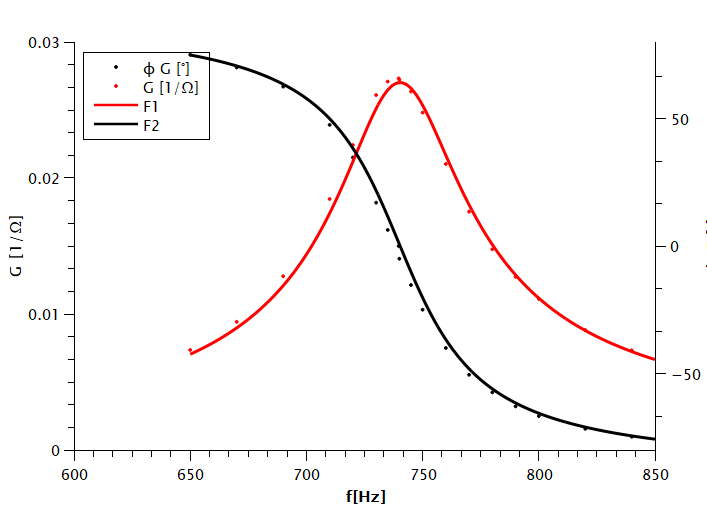
\includegraphics[max width=0.9\linewidth, center]{RLCGphi}
				\caption{Změřená a teoretická závislost velikosti vodivosti a úhlu $\varphi_G$ na frekvenci}
				
			\end{center}
		\end{figure}
		Z fitovacího programu zároveň získáváme data:
		\begin{gather*}
			R = 36.66 \pm 0.11 \,\mathrm{\Omega}\quad L = 110.62 \pm 0.21 \,\mathrm{mH}\\
			C = 420.4 \pm 0.8 \,\mathrm{nF} \quad Q = 13.994 \pm 0.033 \\
			f_0 = 732.02 \pm 0.05 \,\mathrm{Hz} \quad\omega_0 = 4637.1 \pm 0.3 \,\mathrm{rad.s^{-1}}\\
			\alpha = 165.7 \pm 0.4 \,\mathrm{s^{-1}}
		\end{gather*}
		Přičemž hodnota pro $\alpha$ teoreticky vychází \\$\alpha = 136.4 s^{-1}$
\newpage
		
		\subsection{Přechodový jev}
		
		\subsubsection{Podkritické tlumení}
		Měřením získáváme
		\begin{figure}[H]
			\begin{center}
				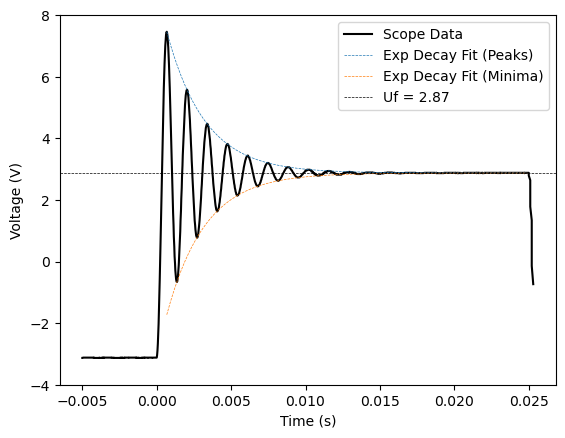
\includegraphics[max width=0.9\linewidth, center]{podkriticke}
				\caption{Závislost napětí na čase při tlumení}\end{center}\end{figure}
		Data jsme proložili křivkami exponenciálního poklesu, z čehož získáváme konstantu $\alpha = 389.6 \pm 0.7$, a jelikož známe $L$, můžeme ze vztahu $2\alpha = \frac R L$ získat hodnotu odporu: $R = 86.2 \pm 0.2 \,\mathrm{\Omega}$.
		
		Tato hodnota je srovnatelná s předpokládaným odporem, jelikož \\$R=R_R + R_G = 36.66 + 50 =86.66$.
		Z formule (33) získáváme $\omega_0 = 4633.97 \pm 0.06\,\mathrm{rad.s^{-1}}$. Pro výpočet frekvence tlumeného kmitání využijeme polohy maxim, které jsme si zjistili pro fitování exponenciální funkcí.
		\subsubsection{Kritické tlumení}
		Ke kritickému tlumení dojde, bude-li platit $\omega_{0} = \frac{R}{2L}$. Proto odpor, při kterém dojde ke kritickému tlumení bude $R=1043 \,\mathrm{\Omega}$.
		Odpor na dekádě zvyšujeme, dokud nepozorujeme vymizení jakékoliv oscilace. K tomu dojde při $R = 955 \,\mathrm{\Omega}$. Získáváme
		\begin{figure}[H]
			\begin{center}
				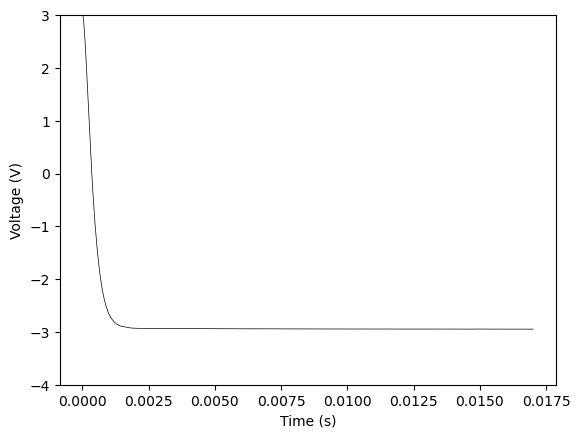
\includegraphics[max width=0.9\linewidth, center]{kriticke}
				\caption{Závislost napětí na čase při tlumení}\end{center}\end{figure}
		Vidíme, že se tento odpor od kalkulovaného liší, je tomu tak nejspíš hlavně proto, že je naprostou absenci na displeji těžké pozorovat. Zde by se hodilo zaznamenávat data s každým zvýšením odporu o $10 \,\mathrm{\Omega}$ a absenci kmitů ověřit numericky. Při bližší analýze dat skutečně pozorujeme, že po poklesu napětí hodnota zprvu dosáhne minima $2.694\,\mathrm{V}$ a až po jednom "překmitu" se ustálí na hodnotě $2.94 \,\mathrm{V}$. U měření pro $R = 1050\,\mathrm{V}$ tyto překmity již skutečně nepozorujeme, je však zbytečné sem vkládat další vizualizaci, jelikož si grafy jsou prakticky identické.
		\subsubsection{Nadkritické tlumení}
		Nyní odpor zvýšíme a pozorujeme chování obvodu:
		\begin{figure}[H]
			\begin{center}
				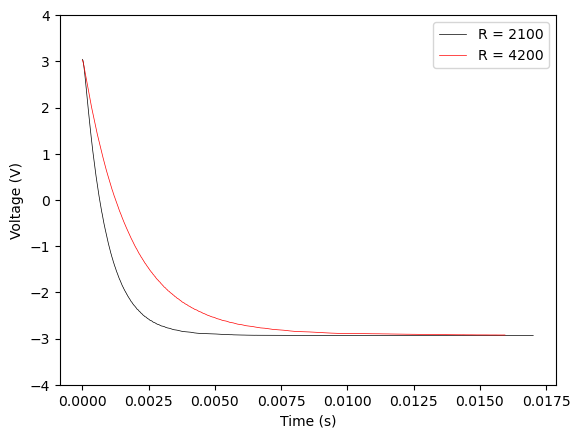
\includegraphics[max width=0.9\linewidth, center]{nadkriticke}
				\caption{Závislost napětí na čase při nadkritickém tlumení}\end{center}\end{figure}
		Z logaritmu rozdílu hodnot napětí a ustálené hodnoty napětí, resp. jejího lineárního fitu, získáme koeficienty $\lambda_{2100} = -1148 \pm0.9, \lambda_{4200} = -572.4 \pm0.2 $, z čehož získáváme hodnoty hodnoty odporů $R_{2100} = 2180 \pm 4\,\mathrm{\Omega},\quad R_{4200} = 4234 \pm 8 \,\mathrm{\Omega}$, které se od skutečných odporů příliš neodchylují.
		
		
		\section{Závěr}
		Podařilo se nám splnit veškeré zadané úkoly a získat hodnoty hledaných veličin. Nepřesnost výsledků části 1(b) vychází patrně z omezené přesnosti měřicího přístroje. 
	
		

		
		
		
		
		
		% Nakonec nezapomeňte projet text programem vlna nebo vlnka, např.
		% 	vlna -m -l -n mojeuloha.tex
		% nebo zkontrolovat a opravit jednopísmenné předložky na koncích řádků ručně.
	\end{multicols}
\end{document}
